% Options for packages loaded elsewhere
\PassOptionsToPackage{unicode}{hyperref}
\PassOptionsToPackage{hyphens}{url}
\PassOptionsToPackage{dvipsnames,svgnames,x11names}{xcolor}
%
\documentclass[
  10pt,
]{scrartcl}
\title{Structured probabilistic coherence \linebreak and the usual counterexamples to probabilistic measures of coherence}
\author{}
\date{\vspace{-2.5em}}

\usepackage{amsmath,amssymb}
\usepackage{lmodern}
\usepackage{iftex}
\ifPDFTeX
  \usepackage[T1]{fontenc}
  \usepackage[utf8]{inputenc}
  \usepackage{textcomp} % provide euro and other symbols
\else % if luatex or xetex
  \usepackage{unicode-math}
  \defaultfontfeatures{Scale=MatchLowercase}
  \defaultfontfeatures[\rmfamily]{Ligatures=TeX,Scale=1}
\fi
% Use upquote if available, for straight quotes in verbatim environments
\IfFileExists{upquote.sty}{\usepackage{upquote}}{}
\IfFileExists{microtype.sty}{% use microtype if available
  \usepackage[]{microtype}
  \UseMicrotypeSet[protrusion]{basicmath} % disable protrusion for tt fonts
}{}
\makeatletter
\@ifundefined{KOMAClassName}{% if non-KOMA class
  \IfFileExists{parskip.sty}{%
    \usepackage{parskip}
  }{% else
    \setlength{\parindent}{0pt}
    \setlength{\parskip}{6pt plus 2pt minus 1pt}}
}{% if KOMA class
  \KOMAoptions{parskip=half}}
\makeatother
\usepackage{xcolor}
\IfFileExists{xurl.sty}{\usepackage{xurl}}{} % add URL line breaks if available
\IfFileExists{bookmark.sty}{\usepackage{bookmark}}{\usepackage{hyperref}}
\hypersetup{
  pdftitle={Structured probabilistic coherence and the usual counterexamples to probabilistic measures of coherence},
  colorlinks=true,
  linkcolor={blue},
  filecolor={blue},
  citecolor={blue},
  urlcolor={blue},
  pdfcreator={LaTeX via pandoc}}
\urlstyle{same} % disable monospaced font for URLs
\usepackage{longtable,booktabs,array}
\usepackage{calc} % for calculating minipage widths
% Correct order of tables after \paragraph or \subparagraph
\usepackage{etoolbox}
\makeatletter
\patchcmd\longtable{\par}{\if@noskipsec\mbox{}\fi\par}{}{}
\makeatother
% Allow footnotes in longtable head/foot
\IfFileExists{footnotehyper.sty}{\usepackage{footnotehyper}}{\usepackage{footnote}}
\makesavenoteenv{longtable}
\usepackage{graphicx}
\makeatletter
\def\maxwidth{\ifdim\Gin@nat@width>\linewidth\linewidth\else\Gin@nat@width\fi}
\def\maxheight{\ifdim\Gin@nat@height>\textheight\textheight\else\Gin@nat@height\fi}
\makeatother
% Scale images if necessary, so that they will not overflow the page
% margins by default, and it is still possible to overwrite the defaults
% using explicit options in \includegraphics[width, height, ...]{}
\setkeys{Gin}{width=\maxwidth,height=\maxheight,keepaspectratio}
% Set default figure placement to htbp
\makeatletter
\def\fps@figure{htbp}
\makeatother
\setlength{\emergencystretch}{3em} % prevent overfull lines
\providecommand{\tightlist}{%
  \setlength{\itemsep}{0pt}\setlength{\parskip}{0pt}}
\setcounter{secnumdepth}{5}
\newlength{\cslhangindent}
\setlength{\cslhangindent}{1.5em}
\newlength{\csllabelwidth}
\setlength{\csllabelwidth}{3em}
\newlength{\cslentryspacingunit} % times entry-spacing
\setlength{\cslentryspacingunit}{\parskip}
\newenvironment{CSLReferences}[2] % #1 hanging-ident, #2 entry spacing
 {% don't indent paragraphs
  \setlength{\parindent}{0pt}
  % turn on hanging indent if param 1 is 1
  \ifodd #1
  \let\oldpar\par
  \def\par{\hangindent=\cslhangindent\oldpar}
  \fi
  % set entry spacing
  \setlength{\parskip}{#2\cslentryspacingunit}
 }%
 {}
\usepackage{calc}
\newcommand{\CSLBlock}[1]{#1\hfill\break}
\newcommand{\CSLLeftMargin}[1]{\parbox[t]{\csllabelwidth}{#1}}
\newcommand{\CSLRightInline}[1]{\parbox[t]{\linewidth - \csllabelwidth}{#1}\break}
\newcommand{\CSLIndent}[1]{\hspace{\cslhangindent}#1}
%\documentclass{article}

% %packages
 \usepackage{booktabs}
\usepackage{subcaption}
\usepackage{multirow}
\usepackage{colortbl}
\usepackage{graphicx}
\usepackage{longtable}
\usepackage{ragged2e}

\usepackage{etex}
%\usepackage{yfonts}
\usepackage{marvosym}
\usepackage[notextcomp]{kpfonts}
\usepackage{nicefrac}
\newcommand*{\QED}{\hfill \footnotesize {\sc Q.e.d.}}
\usepackage{floatrow}
\usepackage[titletoc]{appendix}

\usepackage{tcolorbox}
%\renewcommand\thesubsection{\Alph{subsection}}

\usepackage[textsize=footnotesize]{todonotes}
\newcommand{\ali}[1]{\todo[color=gray!40]{#1}}
\newcommand{\mar}[1]{\todo[color=blue!40]{#1}}
\newcommand{\raf}[1]{\todo[color=olive!40]{#1}}
%\linespread{1.5}


\newcommand{\indep}{\!\perp \!\!\! \perp\!}
\newcommand{\s}[1]{\textsf{#1}}
\newcommand{\ms}[1]{\mathsf{#1}}



\setlength{\parindent}{10pt}
\setlength{\parskip}{1pt}


%language
%\usepackage{times}
\usepackage{mathptmx}
\usepackage[scaled=0.86]{helvet}
\usepackage{t1enc}
%\usepackage[utf8x]{inputenc}
%\usepackage[polish]{babel}
%\usepackage{polski}




%AMS
\usepackage{amsfonts}
\usepackage{amssymb}
\usepackage{amsthm}
\usepackage{amsmath}
\usepackage{mathtools}

\usepackage{geometry}
 \geometry{a4paper,left=35mm,top=20mm,}


%environments
\newtheorem{fact}{Fact}



%abbreviations
\newcommand{\ra}{\rangle}
\newcommand{\la}{\langle}
\newcommand{\n}{\neg}
\newcommand{\et}{\wedge}
\newcommand{\jt}{\rightarrow}
\newcommand{\ko}[1]{\forall  #1\,}
\newcommand{\ro}{\leftrightarrow}
\newcommand{\exi}[1]{\exists\, {_{#1}}}
\newcommand{\pr}[1]{\mathsf{P}(#1)}
\newcommand{\cost}{\mathsf{cost}}
\newcommand{\benefit}{\mathsf{benefit}}
\newcommand{\ut}{\mathsf{ut}}

\newcommand{\odds}{\mathsf{Odds}}
\newcommand{\ind}{\mathsf{Ind}}
\newcommand{\nf}[2]{\nicefrac{#1\,}{#2}}
\newcommand{\R}[1]{\texttt{#1}}
\newcommand{\prr}[1]{\mbox{$\mathtt{P}_{prior}(#1)$}}
\newcommand{\prp}[1]{\mbox{$\mathtt{P}_{posterior}(#1)$}}



\newtheorem{q}{\color{blue}Question}
\newtheorem{lemma}{Lemma}
\newtheorem{theorem}{Theorem}



%technical intermezzo
%---------------------

\newcommand{\intermezzoa}{
	\begin{minipage}[c]{13cm}
	\begin{center}\rule{10cm}{0.4pt}



	\tiny{\sc Optional Content Starts}
	
	\vspace{-1mm}
	
	\rule{10cm}{0.4pt}\end{center}
	\end{minipage}\nopagebreak 
	}


\newcommand{\intermezzob}{\nopagebreak 
	\begin{minipage}[c]{13cm}
	\begin{center}\rule{10cm}{0.4pt}

	\tiny{\sc Optional Content Ends}
	
	\vspace{-1mm}
	
	\rule{10cm}{0.4pt}\end{center}
	\end{minipage}
	}
%--------------------






















\newtheorem*{reply*}{Reply}
\usepackage{enumitem}
\newcommand{\question}[1]{\begin{enumerate}[resume,leftmargin=0cm,labelsep=0cm,align=left]
\item #1
\end{enumerate}}

\usepackage{float}

% \setbeamertemplate{blocks}[rounded][shadow=true]
% \setbeamertemplate{itemize items}[ball]
% \AtBeginPart{}
% \AtBeginSection{}
% \AtBeginSubsection{}
% \AtBeginSubsubsection{}
% \setlength{\emergencystretch}{0em}
% \setlength{\parskip}{0pt}






\usepackage[authoryear]{natbib}

%\bibliographystyle{apalike}



\usepackage{tikz}
\usetikzlibrary{positioning,shapes,arrows}

\usepackage{booktabs}
\usepackage{longtable}
\usepackage{array}
\usepackage{multirow}
\usepackage{wrapfig}
\usepackage{float}
\usepackage{colortbl}
\usepackage{pdflscape}
\usepackage{tabu}
\usepackage{threeparttable}
\usepackage{threeparttablex}
\usepackage[normalem]{ulem}
\usepackage{makecell}
\usepackage{xcolor}
\ifLuaTeX
  \usepackage{selnolig}  % disable illegal ligatures
\fi

\begin{document}
\maketitle

{
\hypersetup{linkcolor=blue}
\setcounter{tocdepth}{3}
\tableofcontents
}
\setlength{\abovedisplayskip}{-10pt}
\setlength{\belowdisplayskip}{5pt}

\pagebreak

\hypertarget{introduction-motivations}{%
\section{Introduction \& motivations}\label{introduction-motivations}}

The notion of coherence is often used in many philosophical, especially epistemological, discussions (for instance, in discussions about the truth-conduciveness of coherence). When we talk about the coherence of a set of propositions or about the coherence of a story, we seem to refer to how well their individual pieces fit together. How are we to understand and apply this notion systematically, though? In particular, we will be interested in probabilistic explications of this notion, as Bayesian epistemology strives to be a general epistemological project and as such it should be able to accommodate coherence-oriented considerations.

There is also a more practical reason to develop a better understanding of the notion: a plausible measure of coherence could be used to better evaluate the quality of some stories or narrations. For example in the legal context we would like to be able to assess the quality of a testimony in the court of law.\\

Multiple probabilistic explications of coherence have been proposed
(Douven \& Meijs, 2007; Fitelson, 2003; Glass, 2002; Meijs \& Douven, 2007; Olsson, 2001; Roche, 2013; Shogenji, 1999). However, clear general principles to choose between them are hard to come by. One paper where some such principles have been formulated is (Schippers, 2014), where a list of seemingly plausible adequacy conditions for a coherence measure is proposed and shown to be inconsistent to argue for pluralism about the notion of coherence. However, some of those requirements are quite non-trivial.\footnote{Let us illustrate this. The (Dependence) condition formulated there requires that the coherence score of a set of propositions is above (below) the neutral score if for all pairs of non-empty subsets the posterior of an element of a pair conditional on the other element is higher than the prior of the former. This makes some of the features of the coherence measure dependent on the priors, and whether it should be so is not obvious. On the other hand, (Agreement) is formulated in terms of conditional probabilities between such pairs. If on a given measure \(\mathsf{P}\) all conditional probabilities (between pairs already mentioned) are higher than on \(\mathsf{P}'\), the coherence of a set given \(\mathsf{P}\) should be higher than given \(\mathsf{P}'\). The (Equivalence) requirement is that any finite set of logically equivalent propositions should be maximally coherent. This is suspicious, as the set \(\{ 0= 1, 2, = 5\}\) is a set of equivalent propositions (with sufficiently strong notion of logical equivalence in the background), but we would intuitively hesitate to say it's maximally coherent.}

The general point here is not that the approach taken in (Schippers, 2014) is flawed, but rather that the task of formulating general principles for coherence is a challenge, and that no clear list of such uncontroversial desiderata is on the horizon.

One approach to obtaining some clarity on which abstract conditions are plausible is looking at various thought experiments in which our intuitions about what the coherence scores should be (at least comparatively) are more robust than direct assessment of general requirements. In fact, looking at examples is what the main stream of literature on probabilistic coherence focused on, and each probabilistic measure of coherence faces a selection of seemingly intuitive counterexamples.

We decided to work with this methodology. We first gathered key examples that occur in the literature, represented them in terms of Bayesian networks, and developed \textbf{\textsf{R}} scripts calculating all coherence scores for the Bayesian networks at play, pushing further the results obtained by Koscholke (2016).\footnote{
  The whole work has been made possible by all those who contributed to the development of \textsf{\textbf{R}} language, and Marco Scutari, the author of \textsf{\textbf{bnlearn}} package, who was kind enough to extend his package with additional features upon our requests (Scutari \& Denis, 2015).} Then we reflected on the results, noticing that one weakness of the measures is that they pay little attention to the underlying structure of a given narration in the calculation of its coherence.

Inspired by this observation, we formulate our own proposal, which diverges from the known purely probabilistic measures of coherence in three important respects: (i) It is not a function of a probability measure and a set
of propositions alone, because it is also sensitive to the selection and direction of edges in a Bayesian network representing an agent's credal state. (ii) Unlike in the case of quite a few coherence measures, it is sensitive to
the weakest links in the narration. (iii) It is not obtained by simply averaging confirmation levels between all possible combinations of elements.

We described this approach in a more detailed introduction to this measure {[}ANONYMIZED{]}, which explains the method and some of the theoretical decisions that we have made, and show how it works using a Bayesian network developed for the well-known Sally Clark case (Fenton \& Neil, 2018). The goal of the current paper is to discuss a range of philosophical counterexamples to the existing probabilistic measures of coherence and evaluate the performance of our approach using those as a benchmark, arguing that it performs much better than the existing ones.

Accordingly, in Section \ref{sec:measures} we introduce all the coherence measures, including the key motivations for and a pseudo-code description of our measure. In Section \ref{sec:examples} we describe the thought experiments meant as counterexamples to coherence measures, their corresponding desiderata and their status on various coherence measures, including ours. The order of the discussion of any given example is straightforward: we first explain what the situation we are to consider is, what the intuitive desiderata related to it are supposed to be, how the situation is represented by means of a Bayesian network(s), and what happens when we apply all coherence measures. We end with Section \ref{sec:discussion} in which we compare all of the results and draw some general conclusions.

\hypertarget{probabilistic-coherence-measures-and-structured-coherence}{%
\section{Probabilistic coherence measures and structured coherence}\label{probabilistic-coherence-measures-and-structured-coherence}}

\label{sec:measures}

Quite a few different measures of coherence have been proposed in the literature. Two early proposals are:

\begin{itemize}
\tightlist
\item
  Shogenji's
  \textbf{deviation from independence} (Shogenji, 1999), is defined as the ratio between the probability of the
  conjunction of all claims, and the probability that the conjunction
  would get if all its conjuncts were probabilistically independent (scaling from 0 to \(\infty\) with neutral point 1):
\end{itemize}

\begin{align}
    \tag{Shogenji}
    \label{coh:Shogenji}
     \mathcal{C}_{S}(S)=\frac{P(\bigwedge S)}{\prod_{i=1}^{\vert S \vert}\{P(S_i)\vert i \in S\}}
\end{align}

\noindent This measure was later generalized by Meijs \& Douven (2007). According to this approach, \eqref{coh:Shogenji} is applied not only to the whole set of propositions, but to each non-empty non-singleton subset of the set, and the final value is defined as the average of all sub-values thus obtained.

\begin{itemize}
\tightlist
\item
  \textbf{Relative overlap} (Glass, 2002; Olsson, 2001), is defined as the ratio between the intersection of all propositions and their union (scaling from -1 to 1 with no clear neutral point):
\end{itemize}

\begin{align}
    \tag{Olsson}
    \label{coh:Olsson}
    \mathcal{C}_{O}(S)=\frac{P(\bigwedge S)}{P(\bigvee S)}
\end{align}

\noindent It has also been generalized in a way analogous to the one used in the generalization of the Shogenji's measure (Meijs \& Douven, 2007).

Both of these approaches are susceptible to various objections and counterexamples (Akiba, 2000; Bovens \& Hartmann, 2004; Crupi, Tentori, \& Gonzalez, 2007; Koscholke, 2016; Merricks, 1995; Schippers \& Koscholke, 2019; Shogenji, 1999, 2001, 2006; Siebel, 2004, 2006). To overcome them, more recent works proposed \textbf{average mutual support} measures, starting with (Fitelson, 2003). The general recipe for such measures is as follows.

\begin{itemize}
\item
  Given that \(S\) is a set whose coherence is to be measured, let \(P\)
  indicate the set of all ordered pairs of non-empty, disjoint subsets
  of \(S\).
\item
  First, define a confirmation function (of  a hypothesis \(H\) by evidence  \(E\)): \(\mathsf{conf}(H,E)\).
\item
  For each pair \(\langle X, Y \rangle \in P\), calculate
  \(\mathsf{conf}(\bigwedge X, \bigwedge Y)\), where $\bigwedge X$  is the conjunction of all the elements of $X$ (and $\bigwedge Y$ is to be understood analogously).
\item
  Take the mean of all the results:
\end{itemize}

\begin{align*}
    \mathcal{C}(S) & =
\mathsf{mean}\left(\left\{\mathsf{conf}(\bigwedge X_i, \bigwedge Y_i) | \langle X_i, Y_i \rangle \in P\right\} \right).
\end{align*}

\noindent Different measures of coherence result from different choices of a confirmation measure. Here are the key candidates present in the literature:

\begin{itemize}
\tightlist
\item
  Fitelson (2003) uses the following confirmation function (the resulting coherence measure ranges from -1 to 1 with neutral point at 0):
\end{itemize}

\begin{align}
    F(H,E) & = \begin{cases}
    1 & E\models H, E\not \models \bot \\
    -1 & E \models \neg H\\
    \frac{P(E|H)-P(E|\neg H)}{P(E|H)+P(E|\neg H)} & \mbox{o/w}
    \end{cases} \nonumber \\
\tag{Fitelson}  
    \mathcal{C}_{F}(S) & =
\mathsf{mean}\left(\left\{F(\bigwedge X_i, \bigwedge Y_i) | \langle X_i, Y_i\rangle \in P\right\} \right)
\end{align}

\begin{itemize}
\tightlist
\item
  Douven \& Meijs (2007) use the difference confirmation measure (with coherence ranging from -1 to 1 with neutral point at 0):
\end{itemize}

\begin{align}
    D(H,E) &= P(H|E) - P(H) \nonumber \\
\tag{DM}  
    \mathcal{C}_{DM}(S) & =
\mathsf{mean}\left(\left\{D(\bigwedge X_i, \bigwedge Y_i) | \langle X_i, Y_i\rangle \in P\right\} \right)
\end{align}

\begin{itemize}
\tightlist
\item
  Roche (2013) uses the absolute confirmation measure
  (the resulting coherence measure ranges from 0 to 1 with neutral point at \(0.5\)):
\end{itemize}

\begin{align} \nonumber 
    A(H,E)  & = \begin{cases}
    1 & E\models H, E\not \models \bot \\
    0 & E \models \neg H\\
    P(H|E) & \mbox{o/w} \\
    \end{cases} \\
\tag{Roche}  
    \mathcal{C}_{R}(S) & =
\mathsf{mean}\left(\left\{A(\bigwedge X_i, \bigwedge Y_i) | \langle X_i, Y_i\rangle \in P\right\} \right) 
\end{align}

Mind your head: different measures use different scales and have different neutral points (values taken for any set of probabilistically independent propositions; not all measures have neutral points). This is worth keeping in mind when it comes to various desiderata that we will discuss.

As we already mentioned in the introduction, formulating abstract formal requirements for a coherence measure and investigating whether a given coherence measure satisfies them has not resulted in an agreement. For this reason, we follow another path, which has dominated the literature on the topic. We look at how the measures behave in test scenarios. Many putative scenarios were put forward as counterexamples. They usually have the form of a few propositions formulated in natural language, such that intuitive judgments of coherence involved and the formal coherence calculations seem to diverge (Akiba, 2000; Bovens \& Hartmann, 2004; Koscholke, 2016; Meijs \& Douven, 2007, 2007; Merricks, 1995; Schippers \& Koscholke, 2019, 2019; Shogenji, 1999, 2001, 2006; Siebel, 2004, 2006). We will focus on these examples in what follows. To spoil the experience, let us already point out that the probabilistic measures we introduced above do not seem to handle these examples very well (read on for details).

Inspired by these failures, in {[}REFERENCE SUPRESSED FOR ANONYMITY{]} we proposed to take a different perspective. Putting the earliest measures aside (they were problematic for various reasons), we noticed that the problems with the average mutual support measures stem from the fact that the coherence score is an average confirmation score for all possible combinations of the parts of a narration. Therefore we proposed to take a more fine-grained account. First, we represented an agent's belief state by means of a Bayesian network, which comprises not only a probabilistic measure but additional structural information, Then we used this structural information in our definition of coherence, so that only those directions of support are considered which in fact are indicated by the structure of the agent's belief state.

While we refer the reader to a more extensive treatment in {[}REFERENCE SUPRESSED FOR ANONYMITY{]}, we now briefly discuss the main idea behind it. A Bayesian network represents agent's probabilistic belief state with respect to the relevant nodes. Some of them are distinguished as fixed narration nodes---the agent holds definite beliefs about which states of these nodes occur.

Each parented node in the BN receives its expected confirmation score (\s{ECS}). It is calculated by looking at all combinations of its states and states of its parents not excluded by agents' fixed beliefs. For each of these combinations, the confirmation score between the parents' states and the child state is calculated (in the pseudo-code, we use confirmation measure \s{Z}, in further calculations we also use measures \s{LR} and \s{L} for comparison)\footnote{DEFINITIONS}. Then, a weighted average of these scores is obtained, where weights are the probabilities of the combinations of parents' states obtained by updating the BN with the fixed states of the fixed narration nodes. The final coherence score is either the mean of the \s{ecs} scores, if all of them are positive, or it is a weighted average of their mean and their minimum, \((1- |\s{min}(\s{ecs})|) \times \s{mean}(\s{ecs}) + |\s{min}(\s{ecs})| \times \s{min}(\s{ecs})\), otherwise.\footnote{We have developed \textbf{\textsf{R}} code calculating this and other measures to handle calculations that will be discussed further on, the code with documentation is available at ANONYMIZED.}

\pagebreak 
\footnotesize

\begin{verbatim}
FUNCTION parents_child_possible_states(parents,child)
    IF child included in narration THEN
        consequentStates <- the unique state of child as reported in the narration
    ELSE
        consequentStates <- all possible states of child
    FOR EACH parent in parents
        IF parent included in narration THEN
            parentStates[parent] <- the unique state of parent as reported in the narration
        ELSE
            parentStates[parent] <- all possible states of parent
    parentsStates <- all combinations of parentStates
    variants <- list of all possible combinations of consequentStates and parentsStates
    RETURN variants


FUNCTION coherence_from_ecs(ecs)
    IF min(ecs) <= 0 THEN
        RETURN mean(ecs) * (min(ecs)+1) - min(ecs)min(ecs)
        #this is equivalent to (1- |min(ecs)|) * mean(ecs) + |min(ecs)| * min(ecs)
    ELSE
        RETURN mean(ecs)

FUNCTION structured_coherence(BN,fixedNodes,fixedStates)
    parentedNodes <- vector of non-root nodes in BN
    ecsList <- []
    FOR EACH parentedNode IN parentedNodes
        variants <- parents_child_possible_states(parents,parentedNode)
        variants_count <- length(variants)
        sumParentsNarr <- 0
        FOR EACH variant IN variants
            childPrior <- prior probability of the child state in variant
            childPosterior <- posterior probability of the child state in variant,
                        obtained by updating on the parents states
                        from this variant
            parentsNarr[variant] <- joint probability of 
                        the parents states in variant in BN updated with fixedStates of fixedNodes
            sumParentsNarr <- sumParentsNarr +  parentsNarr[variant] 
            z[variant] <- z_confirmation_measure(childPrior, childPosterior)
        ecs <- 0  #expected confirmation score
        FOR EACH variant IN variants
            IF parentsNarr[variant] > 0 THEN
                weight <- parentsNarr[variant]/sumParentsNarr
            ELSE
                weight <- 1/variants_count
            zScaled <- z[variant] * weight
            ecs <- ecs + zScaled
        ecsList.add(ecs)
    RETURN coherence_from_ecs(ecsList)
\end{verbatim}

\normalsize

\noindent Having introduced the coherence measures at play, let us now move to the key counterexamples discussed in the literature.

\hypertarget{challenges-and-their-treatment}{%
\section{\texorpdfstring{Challenges and their treatment \label{sec:examples}}{Challenges and their treatment }}\label{challenges-and-their-treatment}}

For each of the counterexamples, we first explain what it is and what the connected desiderata are. Then we represent it as a Bayesian network, and finally we use our \textbf{\textsf{R}} scripts to calculate coherence scores that the coherence measures included in the previous section (including ours) yield for a given example and whether the desiderata are satisfied.
Here are the counterexamples put forward against various coherence measures in the literature. We ignored only a few where both we didn't share the authors' intuitions and the examples were not picked up in further discussion in the literature.

\hypertarget{penguins}{%
\subsection{Penguins}\label{penguins}}

\textbf{The scenario.} A challenge discussed in (Bovens \& Hartmann, 2004, p. 50) and (Meijs \& Douven, 2007) consists of the propositions (instead of \emph{letters} or \emph{abbreviations}, we'll talk about \emph{nodes}, as these will be used later on in Bayesian networks) displayed in Table \ref{tab:penguinsPropositions}.

\begin{table}[H]

\caption{\label{tab:penguinsPropositions}Propositions in the Penguins scenario}
\centering
\begin{tabular}[t]{ll}
\toprule
node & content\\
\midrule
\cellcolor{gray!6}{B} & \cellcolor{gray!6}{Tweety is a bird.}\\
G & Tweety is a grounded animal.\\
\cellcolor{gray!6}{P} & \cellcolor{gray!6}{Tweety is a penguin.}\\
\bottomrule
\end{tabular}
\end{table}

\noindent \textbf{Desiderata.}
It seems that the set \{\s{B},\s{G}\}, which doesn't contain the information about Tweety being a penguin, should be less coherent than the one that does contain this information: \{\s{B},\s{G},\s{P}\}.

\vspace{2mm}\begin{description}
    \item[(\s{BG}$<$\s{BGP})] \{\s{B},\s{G}\}  should be less coherent than \{\s{B},\s{G},\s{P}\}. 
\end{description}\vspace{2mm}

Another intuition about this scenario (Schippers \& Koscholke, 2019) is that when you consider a set which says that Tweety is both a bird and a penguin: \{\s{B},\s{P}\}, adding proposition about not flying (\s{G}) shouldn't increase the coherence of the set as much as moving from \{\s{B},\s{G}\} to \{\s{B},\s{G}, \s{P}\}. It's a well-known fact that penguins don't fly and by adding \s{G} explicitly to the set, one wouldn't gain as much information.
However, as \s{G} is not a logical consequence of \s{P}, it can be argued that \{\s{B},\s{P}\} and \{\s{B},\s{P},\s{G}\} represent different information sets, and so some difference in their coherence is to be expected.

\vspace{2mm}\begin{description}
    \item[(\s{BG} $\ll$ \s{BP}$\leq$\s{BGP})]  \{\s{B},\s{P}\} should be notably above  \{\s{B},\s{G}\}, and less than \{\s{B},\s{P},\s{G}\}.
\end{description}\vspace{2mm}

\noindent Formally, we'll require that the absolute difference between \s{BG} and \s{BP} be greater than \(.1\) (the exact placement of the threshold doesn't make a huge difference, unless it's at an unintuitive value below \(.01\)) and that \{\s{B},\s{G}\} \(\leq\) \{\s{B},\s{P},\s{G}\}.

\noindent \textbf{Bayesian network.} We used the distribution used in the original formulation to build a BN corresponding to the narrations at play (Fig. \ref{fig:BGP}).\footnote{Not without concerns. There are around 18 000 species of birds, and around 60 of them are flightless. We  couldn't find information about counts, but it seems the probability of being a penguin if one is grounded is overestimated by philosophers.  Also, there are many things that are not grounded but are not birds, mostly insects, and there's plenty of them. We did spend some time coming up with plausible ranges of probabilities to correct for such factors, and none of them actually makes a difference to the main point. So, for the sake of simplicity, we leave the original unrealistic distribution in our discussion.}

\begin{figure}[H]
\hspace{2cm}\scalebox{0.7}{\begin{subfigure}[!ht]{0.4\textwidth}

\begin{center}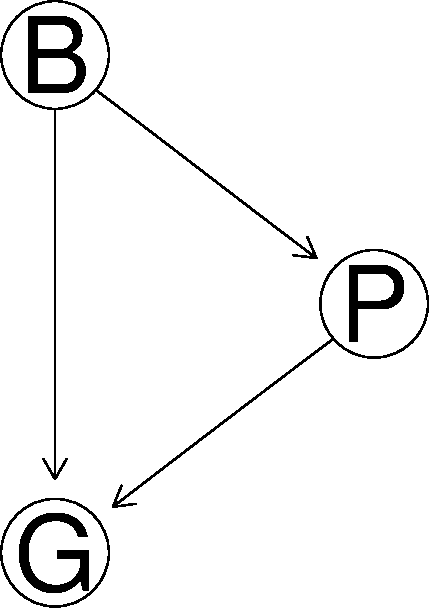
\includegraphics[width=1\linewidth]{coherencePaper35_files/figure-latex/unnamed-chunk-2-1} \end{center}
\end{subfigure}} \hfill
\hspace{-3cm}\scalebox{0.8}{\begin{subfigure}[!ht]{0.4\textwidth}

\begin{tabular}{lr}
\toprule
B & Pr\\
\midrule
1 & 0.5\\
0 & 0.5\\
\bottomrule
\end{tabular}


\begin{tabular}{lrr}
\toprule
\multicolumn{1}{c}{P} & \multicolumn{2}{c}{B} \\
  & 1 & 0\\
\midrule
1 & 0.02 & 0\\
0 & 0.98 & 1\\
\bottomrule
\end{tabular}


\begin{tabular}{lllr}
\toprule
\multicolumn{1}{c}{} & \multicolumn{1}{c}{B} & \multicolumn{1}{c}{P} & \multicolumn{1}{c}{} \\
G &  &  & Pr\\
\midrule
1 & 1 & 1 & 1.00\\
0 & 1 & 1 & 0.00\\
1 & 0 & 1 & 0.00\\
0 & 0 & 1 & 1.00\\
1 & 1 & 0 & 0.00\\
0 & 1 & 0 & 1.00\\
1 & 0 & 0 & 0.98\\
0 & 0 & 0 & 0.02\\
\bottomrule
\end{tabular}
\end{subfigure}}
\caption{Bayesian network for the Penuins problem.}
\label{fig:BGP}
\end{figure}

\begin{figure}[H]
\hspace{2cm}\scalebox{0.6}{
\begin{subfigure}[!ht]{0.4\textwidth}

\begin{center}
\includegraphics[width=0.7\linewidth]{coherencePaper35_files/figure-latex/unnamed-chunk-4-1} \end{center}
\end{subfigure} }
\hfill
\hspace{-3cm}\begin{subfigure}[!ht]{0.4\textwidth}

\begin{tabular}{lr}
\toprule
B & Pr\\
\midrule
1 & 0.5\\
0 & 0.5\\
\bottomrule
\end{tabular}


\begin{tabular}{lrr}
\toprule
\multicolumn{1}{c}{G} & \multicolumn{2}{c}{B} \\
  & 1 & 0\\
\midrule
1 & 0.02 & 0.98\\
0 & 0.98 & 0.02\\
\bottomrule
\end{tabular}
\end{subfigure}
\label{fig-BG}
\caption{Bayesian network for the \textsf{BG} scenario.}
\end{figure}

\begin{figure}[H]
\scalebox{0.6}{
\hspace{4cm}\begin{subfigure}[!ht]{0.4\textwidth}

\begin{center}
\includegraphics{coherencePaper35_files/figure-latex/unnamed-chunk-6-1} \end{center}
\end{subfigure}} \hfill
\hspace{-3cm}\begin{subfigure}[!ht]{0.4\textwidth}

\begin{tabular}{lr}
\toprule
B & Pr\\
\midrule
1 & 0.5\\
0 & 0.5\\
\bottomrule
\end{tabular}


\begin{tabular}{lrr}
\toprule
\multicolumn{1}{c}{P} & \multicolumn{2}{c}{B} \\
  & 1 & 0\\
\midrule
1 & 0.02 & 0\\
0 & 0.98 & 1\\
\bottomrule
\end{tabular}
\end{subfigure}
\caption{Bayesian network for the \textsf{BP} scenario.}
\label{fig:BP}
\end{figure}

\noindent \textbf{Results.} Now, let's calculate the coherence scores (Table \ref{tab:penguinsCoherence}) and see if the desiderata are satisfied (Table \ref{tab:penguinsDesiderata}). The measures are: Olsson-Glass, generalized Olsson-Glass, Shogenji, generalized Shogenji, Douven-Meijs, Roche, Fitelson, Structured with Z, LR, and L used as a confirmation measure.

\begin{table}[H]

\caption{\label{tab:penguinsCoherence}Coherence scores for the Penguins scenario (rounded). Note how LR might result in Inf if a conditional probability of 1 at an arrow used in the calculations is involved.}
\centering
\resizebox{\linewidth}{!}{
\begin{tabular}[t]{lrrrrrrrrrr}
\toprule
  & OG & OGGen & Sh & ShGen & DM & R & Fi & SZ & SLR & SL\\
\midrule
\cellcolor{gray!6}{Penguins: BGP 111} & \cellcolor{gray!6}{0.01} & \cellcolor{gray!6}{0.015} & \cellcolor{gray!6}{4.00} & \cellcolor{gray!6}{2.01} & \cellcolor{gray!6}{0.255} & \cellcolor{gray!6}{0.51} & \cellcolor{gray!6}{0.453} & \cellcolor{gray!6}{0.505} & \cellcolor{gray!6}{Inf} & \cellcolor{gray!6}{0.669}\\
Penguins: BG 11 & 0.01 & 0.010 & 0.04 & 0.04 & -0.480 & 0.02 & -0.960 & -0.960 & 0.02 & -0.960\\
\cellcolor{gray!6}{Penguins: BP 11} & \cellcolor{gray!6}{0.02} & \cellcolor{gray!6}{0.020} & \cellcolor{gray!6}{2.00} & \cellcolor{gray!6}{2.00} & \cellcolor{gray!6}{0.255} & \cellcolor{gray!6}{0.51} & \cellcolor{gray!6}{0.669} & \cellcolor{gray!6}{0.010} & \cellcolor{gray!6}{2.02} & \cellcolor{gray!6}{0.338}\\
\bottomrule
\end{tabular}}
\end{table}

\begin{table}[H]

\caption{\label{tab:penguinsDesiderata}Desiderata satisfaction for the Penguins scenario.}
\centering
\resizebox{\linewidth}{!}{
\begin{tabular}[t]{lllllllllll}
\toprule
  & OG & OGGen & Sh & ShGen & DM & R & Fi & SZ & SLR & SL\\
\midrule
\cellcolor{gray!6}{Penguins: BG$<$BGP} & \cellcolor{gray!6}{FALSE} & \cellcolor{gray!6}{TRUE} & \cellcolor{gray!6}{TRUE} & \cellcolor{gray!6}{TRUE} & \cellcolor{gray!6}{TRUE} & \cellcolor{gray!6}{TRUE} & \cellcolor{gray!6}{TRUE} & \cellcolor{gray!6}{TRUE} & \cellcolor{gray!6}{TRUE} & \cellcolor{gray!6}{TRUE}\\
Penguins: BG$<<$ BP$<$ BGP & FALSE & FALSE & TRUE & TRUE & TRUE & TRUE & TRUE & TRUE & TRUE & TRUE\\
\bottomrule
\end{tabular}}
\end{table}

\hypertarget{references}{%
\section*{References}\label{references}}
\addcontentsline{toc}{section}{References}

\hypertarget{refs}{}
\begin{CSLReferences}{1}{0}
\leavevmode\vadjust pre{\hypertarget{ref-Akiba2000Shogenjis}{}}%
Akiba, K. (2000). Shogenji's probabilistic measure of coherence is incoherent. \emph{Analysis}, \emph{60}(4), 356--359. \url{https://doi.org/10.1093/analys/60.4.356}

\leavevmode\vadjust pre{\hypertarget{ref-bovens2004bayesian}{}}%
Bovens, L., \& Hartmann, S. (2004). \emph{Bayesian epistemology}. Oxford University Press.

\leavevmode\vadjust pre{\hypertarget{ref-crupi2007BayesianMeasuresEvidential}{}}%
Crupi, V., Tentori, K., \& Gonzalez, M. (2007). On {Bayesian measures} of {evidential Support}: {theoretical} and {empirical Issues}. \emph{Philosophy of Science}, \emph{74}(2), 229--252. \url{https://doi.org/10.1086/520779}

\leavevmode\vadjust pre{\hypertarget{ref-Douven2007measuring}{}}%
Douven, I., \& Meijs, W. (2007). Measuring coherence. \emph{Synthese}, \emph{156}(3), 405--425. \url{https://doi.org/10.1007/s11229-006-9131-z}

\leavevmode\vadjust pre{\hypertarget{ref-Fenton2018Risk}{}}%
Fenton, N., \& Neil, M. (2018). \emph{Risk assessment and decision analysis with bayesian networks}. Chapman; Hall.

\leavevmode\vadjust pre{\hypertarget{ref-fitelson2003ProbabilisticTheoryCoherence}{}}%
Fitelson, B. (2003). A {Probabilistic Theory} of {Coherence}. \emph{Analysis}, \emph{63}(3), 194--199.

\leavevmode\vadjust pre{\hypertarget{ref-glass2002}{}}%
Glass, D. H. (2002). Coherence, {Explanation}, and {Bayesian Networks}. In G. Goos, J. Hartmanis, J. van Leeuwen, M. O'Neill, R. F. E. Sutcliffe, C. Ryan, \ldots{} N. J. L. Griffith (Eds.), \emph{Artificial {Intelligence} and {Cognitive Science}} (Vol. 2464, pp. 177--182). {Berlin, Heidelberg}: {Springer Berlin Heidelberg}. \url{https://doi.org/10.1007/3-540-45750-X_23}

\leavevmode\vadjust pre{\hypertarget{ref-koscholke2016evaluating}{}}%
Koscholke, J. (2016). Evaluating test cases for probabilistic measures of coherence. \emph{Erkenntnis}, \emph{81}(1), 155--181. \url{https://doi.org/10.1007/s10670-015-9734-1}

\leavevmode\vadjust pre{\hypertarget{ref-Meijs2007Alleged}{}}%
Meijs, W., \& Douven, I. (2007). On the alleged impossibility of coherence. \emph{Synthese}, \emph{157}(3), 347--360. \url{https://doi.org/10.1007/s11229-006-9060-x}

\leavevmode\vadjust pre{\hypertarget{ref-Merricks1995}{}}%
Merricks, T. (1995). Warrant entails truth. \emph{Philosophy and Phenomenological Research}, \emph{55}, 841--855.

\leavevmode\vadjust pre{\hypertarget{ref-olsson2001conducive}{}}%
Olsson, E. J. (2001). Why {Coherence Is Not Truth}-{Conducive}. \emph{Analysis}, \emph{61}(3), 236--241.

\leavevmode\vadjust pre{\hypertarget{ref-Roche2013Coherence}{}}%
Roche, W. (2013). Coherence and probability: A probabilistic account of coherence. In M. Araszkiewicz \& J. Savelka (Eds.), \emph{Coherence: Insights from philosophy, jurisprudence and artificial intelligence} (pp. 59--91). Dordrecht: Springer.

\leavevmode\vadjust pre{\hypertarget{ref-Schippers2014Probabilistic}{}}%
Schippers, M. (2014). \emph{Probabilistic measures of coherence: From adequacy constraints towards pluralism}. \emph{191}(16), 3821--3845. \url{https://doi.org/10.1007/s11229-014-0501-7}

\leavevmode\vadjust pre{\hypertarget{ref-Schippers2019General}{}}%
Schippers, M., \& Koscholke, J. (2019). A {General Framework} for {Probabilistic Measures} of {Coherence}. \emph{Studia Logica}. \url{https://doi.org/10.1007/s11225-019-09848-3}

\leavevmode\vadjust pre{\hypertarget{ref-Scutari2015Bayesian-Networ}{}}%
Scutari, M., \& Denis, J.-B. (2015). \emph{Bayesian networks in \textbf{{r}}}. CRC Press.

\leavevmode\vadjust pre{\hypertarget{ref-shogenji1999conducive}{}}%
Shogenji, T. (1999). Is coherence truth-conducive? \emph{Analysis}, \emph{59}(4), 338--345.

\leavevmode\vadjust pre{\hypertarget{ref-Shogenji2001Reply}{}}%
Shogenji, T. (2001). Reply to {A}kiba on the probabilistic measure of coherence. \emph{Analysis}, \emph{61}(2), 147--150. \url{https://doi.org/10.1093/analys/61.2.147}

\leavevmode\vadjust pre{\hypertarget{ref-Shogenji2006Why}{}}%
Shogenji, T. (2006). Why does coherence appear truth-conducive? \emph{Synthese}, \emph{157}(3), 361--372. \url{https://doi.org/10.1007/s11229-006-9062-8}

\leavevmode\vadjust pre{\hypertarget{ref-Siebel2004On-Fitelsons-me}{}}%
Siebel, M. (2004). On {F}itelson's measure of coherence. \emph{Analysis}, \emph{64}, 189--190.

\leavevmode\vadjust pre{\hypertarget{ref-siebel2006against}{}}%
Siebel, M. (2006). Against probabilistic measures of coherence. In \emph{Coherence, truth and testimony} (pp. 43--68). Springer.

\end{CSLReferences}

\end{document}
